%
% file: localoperator.tex
% author: Victor Brena
% description: Briefly describes properties of the local operator.
%

\chapter{Appendix A}\label{app:app01}
\section*{Two Way Ranging (TWR)} % TODO: Look at pulling this put into an appendix?
TWR is a ranging method that utilises TOF and delays during transmission of a packet in order to determine the range between a tag and anchor.
Figure~\ref{fig:twr} provides a simple illustration of how this works.
The distance for an individual tag and an anchor can be obtained by:
\[
    d=c.\frac{(TT2-TT1)-(TA2-TA2)}{2}
\]
This is repeated for each anchor and then the position of the tag can be determined via trilateration.
Geometrically, the position of the tag can be described as the point intersection of all the circles with distance,d , from the tag.
This can be seen in Figure~\ref{fig:trilat}.
\begin{figure}[h!]
    \centering
    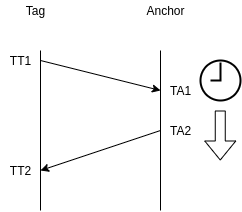
\includegraphics[scale=.7]{lr/TWR}
    \caption{Packet transfer in TWR.}
    \label{fig:twr}
\end{figure}

\begin{figure}[h!]
    \centering
    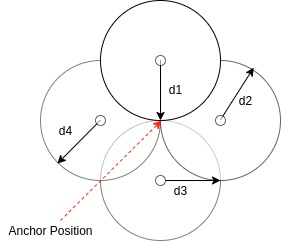
\includegraphics[scale=.7]{lr/trilat}
    \caption{4 Anchor and 1 Tag trilateration in 2D.}
    \label{fig:trilat}
\end{figure}
\newpage

\section*{Sensor Fusion}
From the previous section we have described the basic principle of operation of the Pozyx system.
With a tag we are able to at least determine a rough estimate of the position of a tag in a given reference frame.
Additionally, the tag has an Inertial Measurement Unit (IMU), consisting of an Accelerometer, Gyroscope and Magnetometer, and an Altimeter.
These are used in one of the operational modes of the Pozyx system in order to improve accuracy.
The idea of sensor fusion is to combine multiple sources of data in order to get a fairly accurate estimate of the pose of the system,
The measurements from the tag can be combined with the sensors onward a FCU in order to achieve this.
The de-facto sensor fusion technique is called the Extended Kalman Filter (EKF).
~\citet{simpleekf} present a useful description and example of how the EKF works.
Algorithmically, the EKF is a recursive process using predictions based on the dynamics of the vehicles and updating the estimate based on these predictions and measurements from various sources.
The major requirement for the EKF is that the process model and the measurement model are differentiable.
The steps for the EKF are as follows:
\begin{enumerate}
    \item Provide and initial estimate for the state, $\hat{x}^+_k$, and the prediction error, $P^+_k$.
    \item Compute the Kalman gain, $K_k = P^+_{k}H_k^T(H_k P^+_{k}H_k^T + R)^{-1}$
    \item Update the estimate with measurement $z_k$, $\hat{x}_k=\hat{x}^+_k + K_k(z_k - h(\hat{x}^+_k))$
    \item Update the prediction error, $P_k = (I - K_k H_k)P^+_{k}$
    \item Project the state ahead, $\hat{x}^+_{k+1} = f(\hat{x}_k, u_k, w)$
    \item Project the Prediction error ahead, $P^+_{k+1} = A_k P_k A_k^T + Q_k$
    \item Repeat from step 2.
\end{enumerate}
Where K is the Kalman gain, R is the Measurement Noise Covariance Matrix, Q is the Process Noise Covariance matrix.









